\section{实验结果及分析}

\subsection{ALU验证实验结果}
仿真时 num2（操作数 B）固定为 \texttt{32'h00000001}，num1（操作数 A）按下表输入，验证全部 6 种运算功能，结果均正确。

\begin{table}[htbp]
    \centering
    \begin{tabular}{c|c|c}
        操作            &   Num1         &   Result \\ \hline
        A + B(Unsigned) &   8'b00000010  &   8'b00000011 \\
        A - B           &   8'b11111111  &   8'b11111110 \\
        A AND B         &   8'b11111110  &   8'b00000000 \\
        A OR B          &   8'b10101010  &   8'b10101011 \\
        $\overline{A}$  &   8'b11110000  &   32'hFFFFFF0F \\
        SLT             &   8'b10000001  &   8'b00000000 \\ \hline
    \end{tabular}
    \caption{ALU结果表}
    \label{tab:alu_result}
\end{table}

\textbf{分析：}ALU为纯组合逻辑，每次输入变化后结果立即更新，无时钟延迟。SLT操作中 num1=0x81=129（无符号），作为有符号32位数仍为正数129，大于 num2=1，故输出0。

\subsection{流水线阻塞（暂停）仿真图}

\begin{figure}[htbp]
    \centering
    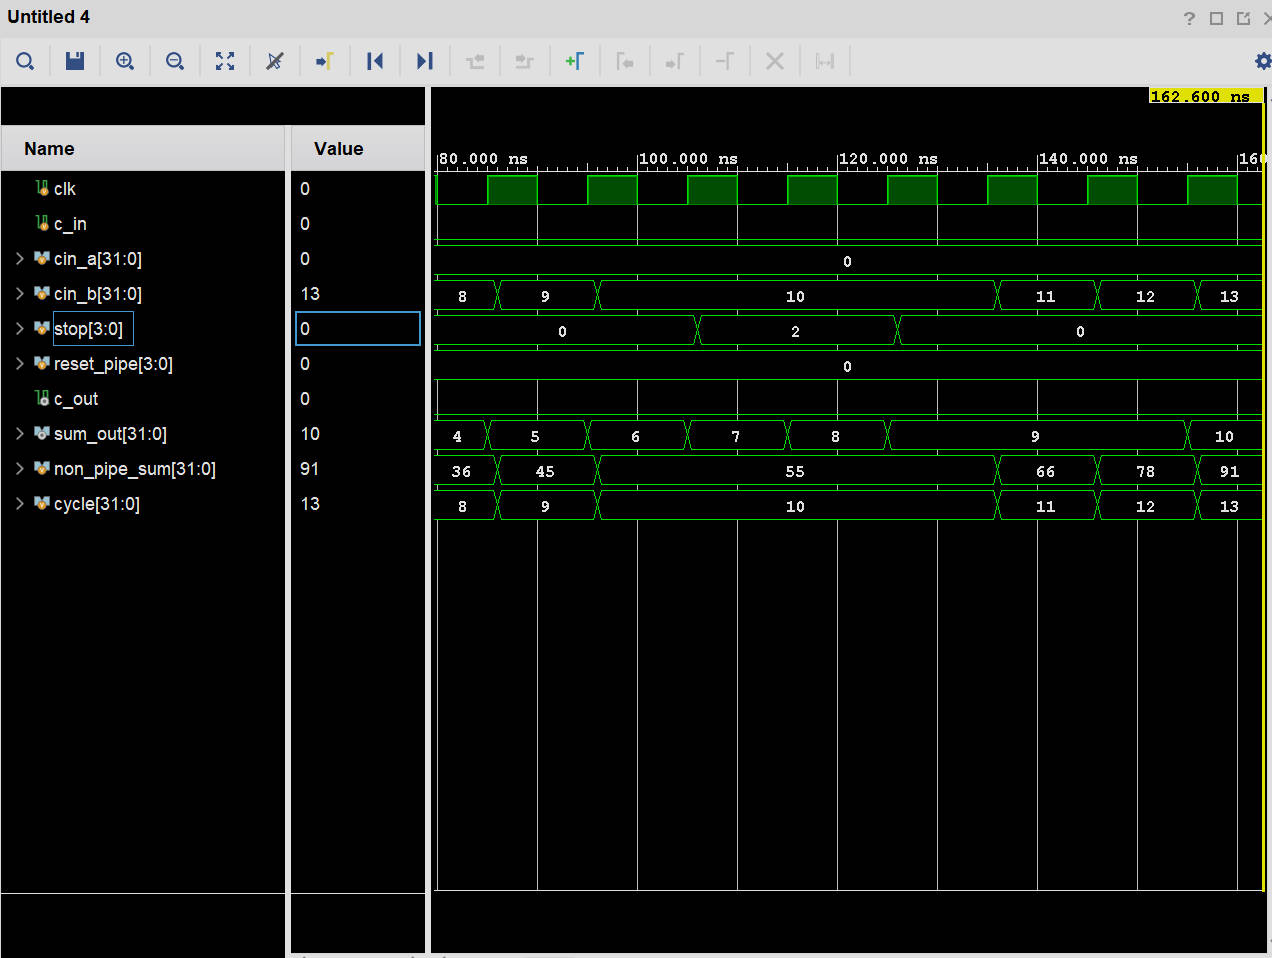
\includegraphics[width=0.85\textwidth]{image/stall.png}
    \caption{流水线阻塞（暂停）仿真波形}
    \label{fig:stall}
\end{figure}

\textbf{分析：}第10个周期时 stop[1] 拉高持续2个周期，第2级流水线寄存器保持当前值不更新，sum\_out 输出冻结，可观察到流水线暂停现象。non\_pipe\_sum 作为非流水线行为级对比，每拍即时更新，体现了流水线与非流水线在时序响应上的差异。

\subsection{流水线刷新（清空）仿真图}

\begin{figure}[htbp]
    \centering
    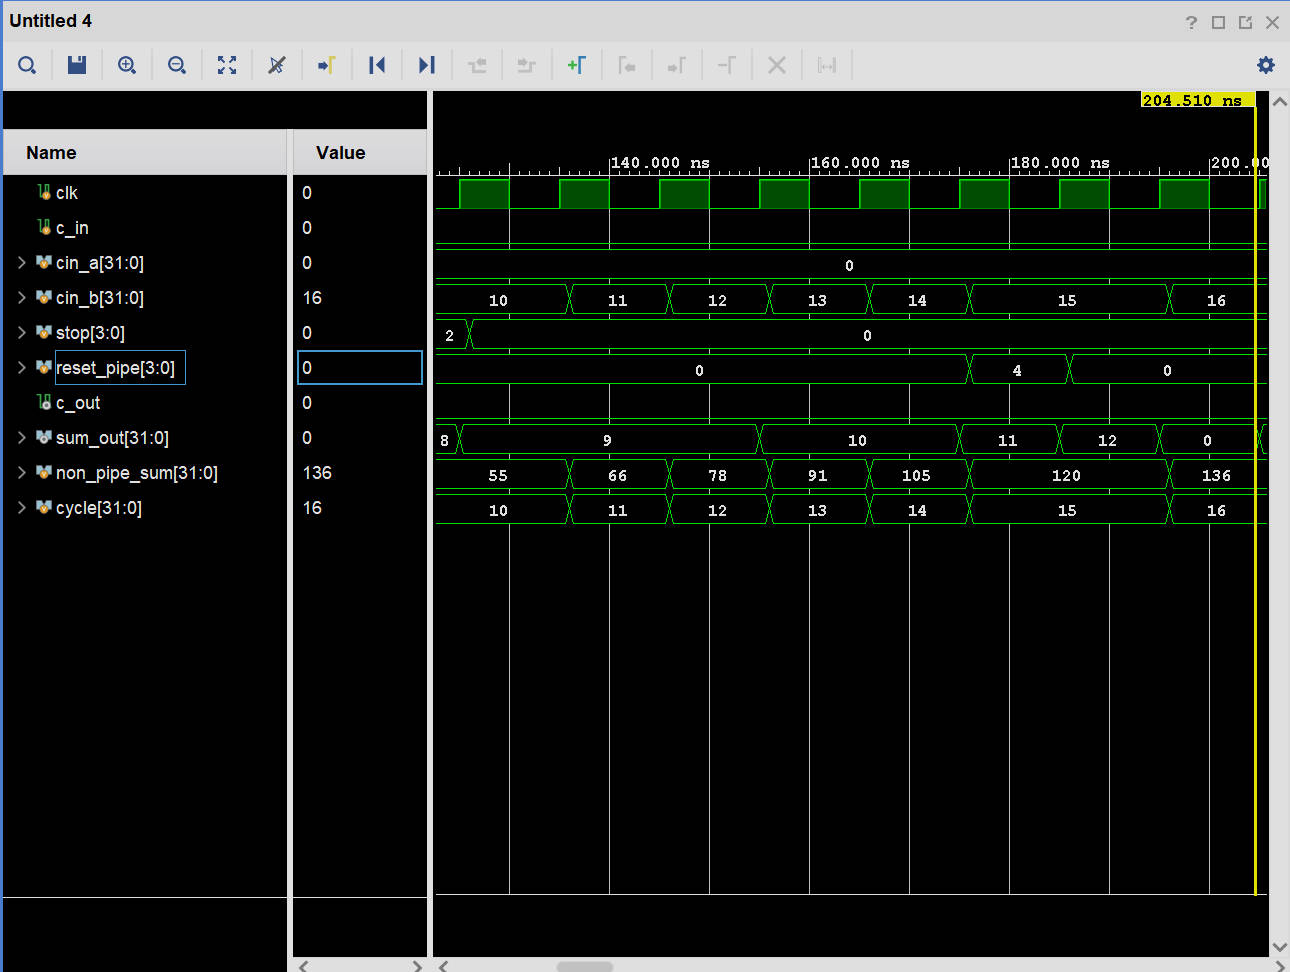
\includegraphics[width=0.85\textwidth]{image/flush.png}
    \caption{流水线刷新（清空）仿真波形}
    \label{fig:flush}
\end{figure}

\textbf{分析：}第15个周期时 reset[2] 拉高一个周期，第3级流水线寄存器被清零，对应级的中间结果丢失，sum\_out 输出出现对应的数据断层，模拟了流水线刷新（清空）的行为，例如 CPU 中分支预测失败时的流水线清空场景。
